\documentclass[11pt]{article}

    \usepackage[breakable]{tcolorbox}
    \usepackage{parskip} % Stop auto-indenting (to mimic markdown behaviour)
    
    \usepackage{iftex}
    \ifPDFTeX
    	\usepackage[T1]{fontenc}
    	\usepackage{mathpazo}
    \else
    	\usepackage{fontspec}
    \fi

    % Basic figure setup, for now with no caption control since it's done
    % automatically by Pandoc (which extracts ![](path) syntax from Markdown).
    \usepackage{graphicx}
    % Maintain compatibility with old templates. Remove in nbconvert 6.0
    \let\Oldincludegraphics\includegraphics
    % Ensure that by default, figures have no caption (until we provide a
    % proper Figure object with a Caption API and a way to capture that
    % in the conversion process - todo).
    \usepackage{caption}
    \DeclareCaptionFormat{nocaption}{}
    \captionsetup{format=nocaption,aboveskip=0pt,belowskip=0pt}

    \usepackage{float}
    \floatplacement{figure}{H} % forces figures to be placed at the correct location
    \usepackage{xcolor} % Allow colors to be defined
    \usepackage{enumerate} % Needed for markdown enumerations to work
    \usepackage{geometry} % Used to adjust the document margins
    \usepackage{amsmath} % Equations
    \usepackage{amssymb} % Equations
    \usepackage{textcomp} % defines textquotesingle
    % Hack from http://tex.stackexchange.com/a/47451/13684:
    \AtBeginDocument{%
        \def\PYZsq{\textquotesingle}% Upright quotes in Pygmentized code
    }
    \usepackage{upquote} % Upright quotes for verbatim code
    \usepackage{eurosym} % defines \euro
    \usepackage[mathletters]{ucs} % Extended unicode (utf-8) support
    \usepackage{fancyvrb} % verbatim replacement that allows latex
    \usepackage{grffile} % extends the file name processing of package graphics 
                         % to support a larger range
    \makeatletter % fix for old versions of grffile with XeLaTeX
    \@ifpackagelater{grffile}{2019/11/01}
    {
      % Do nothing on new versions
    }
    {
      \def\Gread@@xetex#1{%
        \IfFileExists{"\Gin@base".bb}%
        {\Gread@eps{\Gin@base.bb}}%
        {\Gread@@xetex@aux#1}%
      }
    }
    \makeatother
    \usepackage[Export]{adjustbox} % Used to constrain images to a maximum size
    \adjustboxset{max size={0.9\linewidth}{0.9\paperheight}}

    % The hyperref package gives us a pdf with properly built
    % internal navigation ('pdf bookmarks' for the table of contents,
    % internal cross-reference links, web links for URLs, etc.)
    \usepackage{hyperref}
    % The default LaTeX title has an obnoxious amount of whitespace. By default,
    % titling removes some of it. It also provides customization options.
    \usepackage{titling}
    \usepackage{longtable} % longtable support required by pandoc >1.10
    \usepackage{booktabs}  % table support for pandoc > 1.12.2
    \usepackage[inline]{enumitem} % IRkernel/repr support (it uses the enumerate* environment)
    \usepackage[normalem]{ulem} % ulem is needed to support strikethroughs (\sout)
                                % normalem makes italics be italics, not underlines
    \usepackage{mathrsfs}
    

    
    % Colors for the hyperref package
    \definecolor{urlcolor}{rgb}{0,.145,.698}
    \definecolor{linkcolor}{rgb}{.71,0.21,0.01}
    \definecolor{citecolor}{rgb}{.12,.54,.11}

    % ANSI colors
    \definecolor{ansi-black}{HTML}{3E424D}
    \definecolor{ansi-black-intense}{HTML}{282C36}
    \definecolor{ansi-red}{HTML}{E75C58}
    \definecolor{ansi-red-intense}{HTML}{B22B31}
    \definecolor{ansi-green}{HTML}{00A250}
    \definecolor{ansi-green-intense}{HTML}{007427}
    \definecolor{ansi-yellow}{HTML}{DDB62B}
    \definecolor{ansi-yellow-intense}{HTML}{B27D12}
    \definecolor{ansi-blue}{HTML}{208FFB}
    \definecolor{ansi-blue-intense}{HTML}{0065CA}
    \definecolor{ansi-magenta}{HTML}{D160C4}
    \definecolor{ansi-magenta-intense}{HTML}{A03196}
    \definecolor{ansi-cyan}{HTML}{60C6C8}
    \definecolor{ansi-cyan-intense}{HTML}{258F8F}
    \definecolor{ansi-white}{HTML}{C5C1B4}
    \definecolor{ansi-white-intense}{HTML}{A1A6B2}
    \definecolor{ansi-default-inverse-fg}{HTML}{FFFFFF}
    \definecolor{ansi-default-inverse-bg}{HTML}{000000}

    % common color for the border for error outputs.
    \definecolor{outerrorbackground}{HTML}{FFDFDF}

    % commands and environments needed by pandoc snippets
    % extracted from the output of `pandoc -s`
    \providecommand{\tightlist}{%
      \setlength{\itemsep}{0pt}\setlength{\parskip}{0pt}}
    \DefineVerbatimEnvironment{Highlighting}{Verbatim}{commandchars=\\\{\}}
    % Add ',fontsize=\small' for more characters per line
    \newenvironment{Shaded}{}{}
    \newcommand{\KeywordTok}[1]{\textcolor[rgb]{0.00,0.44,0.13}{\textbf{{#1}}}}
    \newcommand{\DataTypeTok}[1]{\textcolor[rgb]{0.56,0.13,0.00}{{#1}}}
    \newcommand{\DecValTok}[1]{\textcolor[rgb]{0.25,0.63,0.44}{{#1}}}
    \newcommand{\BaseNTok}[1]{\textcolor[rgb]{0.25,0.63,0.44}{{#1}}}
    \newcommand{\FloatTok}[1]{\textcolor[rgb]{0.25,0.63,0.44}{{#1}}}
    \newcommand{\CharTok}[1]{\textcolor[rgb]{0.25,0.44,0.63}{{#1}}}
    \newcommand{\StringTok}[1]{\textcolor[rgb]{0.25,0.44,0.63}{{#1}}}
    \newcommand{\CommentTok}[1]{\textcolor[rgb]{0.38,0.63,0.69}{\textit{{#1}}}}
    \newcommand{\OtherTok}[1]{\textcolor[rgb]{0.00,0.44,0.13}{{#1}}}
    \newcommand{\AlertTok}[1]{\textcolor[rgb]{1.00,0.00,0.00}{\textbf{{#1}}}}
    \newcommand{\FunctionTok}[1]{\textcolor[rgb]{0.02,0.16,0.49}{{#1}}}
    \newcommand{\RegionMarkerTok}[1]{{#1}}
    \newcommand{\ErrorTok}[1]{\textcolor[rgb]{1.00,0.00,0.00}{\textbf{{#1}}}}
    \newcommand{\NormalTok}[1]{{#1}}
    
    % Additional commands for more recent versions of Pandoc
    \newcommand{\ConstantTok}[1]{\textcolor[rgb]{0.53,0.00,0.00}{{#1}}}
    \newcommand{\SpecialCharTok}[1]{\textcolor[rgb]{0.25,0.44,0.63}{{#1}}}
    \newcommand{\VerbatimStringTok}[1]{\textcolor[rgb]{0.25,0.44,0.63}{{#1}}}
    \newcommand{\SpecialStringTok}[1]{\textcolor[rgb]{0.73,0.40,0.53}{{#1}}}
    \newcommand{\ImportTok}[1]{{#1}}
    \newcommand{\DocumentationTok}[1]{\textcolor[rgb]{0.73,0.13,0.13}{\textit{{#1}}}}
    \newcommand{\AnnotationTok}[1]{\textcolor[rgb]{0.38,0.63,0.69}{\textbf{\textit{{#1}}}}}
    \newcommand{\CommentVarTok}[1]{\textcolor[rgb]{0.38,0.63,0.69}{\textbf{\textit{{#1}}}}}
    \newcommand{\VariableTok}[1]{\textcolor[rgb]{0.10,0.09,0.49}{{#1}}}
    \newcommand{\ControlFlowTok}[1]{\textcolor[rgb]{0.00,0.44,0.13}{\textbf{{#1}}}}
    \newcommand{\OperatorTok}[1]{\textcolor[rgb]{0.40,0.40,0.40}{{#1}}}
    \newcommand{\BuiltInTok}[1]{{#1}}
    \newcommand{\ExtensionTok}[1]{{#1}}
    \newcommand{\PreprocessorTok}[1]{\textcolor[rgb]{0.74,0.48,0.00}{{#1}}}
    \newcommand{\AttributeTok}[1]{\textcolor[rgb]{0.49,0.56,0.16}{{#1}}}
    \newcommand{\InformationTok}[1]{\textcolor[rgb]{0.38,0.63,0.69}{\textbf{\textit{{#1}}}}}
    \newcommand{\WarningTok}[1]{\textcolor[rgb]{0.38,0.63,0.69}{\textbf{\textit{{#1}}}}}
    
    
    % Define a nice break command that doesn't care if a line doesn't already
    % exist.
    \def\br{\hspace*{\fill} \\* }
    % Math Jax compatibility definitions
    \def\gt{>}
    \def\lt{<}
    \let\Oldtex\TeX
    \let\Oldlatex\LaTeX
    \renewcommand{\TeX}{\textrm{\Oldtex}}
    \renewcommand{\LaTeX}{\textrm{\Oldlatex}}
    % Document parameters
    % Document title
    \title{PCLab1\_Grupo10}
    
    
    
    
    
% Pygments definitions
\makeatletter
\def\PY@reset{\let\PY@it=\relax \let\PY@bf=\relax%
    \let\PY@ul=\relax \let\PY@tc=\relax%
    \let\PY@bc=\relax \let\PY@ff=\relax}
\def\PY@tok#1{\csname PY@tok@#1\endcsname}
\def\PY@toks#1+{\ifx\relax#1\empty\else%
    \PY@tok{#1}\expandafter\PY@toks\fi}
\def\PY@do#1{\PY@bc{\PY@tc{\PY@ul{%
    \PY@it{\PY@bf{\PY@ff{#1}}}}}}}
\def\PY#1#2{\PY@reset\PY@toks#1+\relax+\PY@do{#2}}

\expandafter\def\csname PY@tok@w\endcsname{\def\PY@tc##1{\textcolor[rgb]{0.73,0.73,0.73}{##1}}}
\expandafter\def\csname PY@tok@c\endcsname{\let\PY@it=\textit\def\PY@tc##1{\textcolor[rgb]{0.25,0.50,0.50}{##1}}}
\expandafter\def\csname PY@tok@cp\endcsname{\def\PY@tc##1{\textcolor[rgb]{0.74,0.48,0.00}{##1}}}
\expandafter\def\csname PY@tok@k\endcsname{\let\PY@bf=\textbf\def\PY@tc##1{\textcolor[rgb]{0.00,0.50,0.00}{##1}}}
\expandafter\def\csname PY@tok@kp\endcsname{\def\PY@tc##1{\textcolor[rgb]{0.00,0.50,0.00}{##1}}}
\expandafter\def\csname PY@tok@kt\endcsname{\def\PY@tc##1{\textcolor[rgb]{0.69,0.00,0.25}{##1}}}
\expandafter\def\csname PY@tok@o\endcsname{\def\PY@tc##1{\textcolor[rgb]{0.40,0.40,0.40}{##1}}}
\expandafter\def\csname PY@tok@ow\endcsname{\let\PY@bf=\textbf\def\PY@tc##1{\textcolor[rgb]{0.67,0.13,1.00}{##1}}}
\expandafter\def\csname PY@tok@nb\endcsname{\def\PY@tc##1{\textcolor[rgb]{0.00,0.50,0.00}{##1}}}
\expandafter\def\csname PY@tok@nf\endcsname{\def\PY@tc##1{\textcolor[rgb]{0.00,0.00,1.00}{##1}}}
\expandafter\def\csname PY@tok@nc\endcsname{\let\PY@bf=\textbf\def\PY@tc##1{\textcolor[rgb]{0.00,0.00,1.00}{##1}}}
\expandafter\def\csname PY@tok@nn\endcsname{\let\PY@bf=\textbf\def\PY@tc##1{\textcolor[rgb]{0.00,0.00,1.00}{##1}}}
\expandafter\def\csname PY@tok@ne\endcsname{\let\PY@bf=\textbf\def\PY@tc##1{\textcolor[rgb]{0.82,0.25,0.23}{##1}}}
\expandafter\def\csname PY@tok@nv\endcsname{\def\PY@tc##1{\textcolor[rgb]{0.10,0.09,0.49}{##1}}}
\expandafter\def\csname PY@tok@no\endcsname{\def\PY@tc##1{\textcolor[rgb]{0.53,0.00,0.00}{##1}}}
\expandafter\def\csname PY@tok@nl\endcsname{\def\PY@tc##1{\textcolor[rgb]{0.63,0.63,0.00}{##1}}}
\expandafter\def\csname PY@tok@ni\endcsname{\let\PY@bf=\textbf\def\PY@tc##1{\textcolor[rgb]{0.60,0.60,0.60}{##1}}}
\expandafter\def\csname PY@tok@na\endcsname{\def\PY@tc##1{\textcolor[rgb]{0.49,0.56,0.16}{##1}}}
\expandafter\def\csname PY@tok@nt\endcsname{\let\PY@bf=\textbf\def\PY@tc##1{\textcolor[rgb]{0.00,0.50,0.00}{##1}}}
\expandafter\def\csname PY@tok@nd\endcsname{\def\PY@tc##1{\textcolor[rgb]{0.67,0.13,1.00}{##1}}}
\expandafter\def\csname PY@tok@s\endcsname{\def\PY@tc##1{\textcolor[rgb]{0.73,0.13,0.13}{##1}}}
\expandafter\def\csname PY@tok@sd\endcsname{\let\PY@it=\textit\def\PY@tc##1{\textcolor[rgb]{0.73,0.13,0.13}{##1}}}
\expandafter\def\csname PY@tok@si\endcsname{\let\PY@bf=\textbf\def\PY@tc##1{\textcolor[rgb]{0.73,0.40,0.53}{##1}}}
\expandafter\def\csname PY@tok@se\endcsname{\let\PY@bf=\textbf\def\PY@tc##1{\textcolor[rgb]{0.73,0.40,0.13}{##1}}}
\expandafter\def\csname PY@tok@sr\endcsname{\def\PY@tc##1{\textcolor[rgb]{0.73,0.40,0.53}{##1}}}
\expandafter\def\csname PY@tok@ss\endcsname{\def\PY@tc##1{\textcolor[rgb]{0.10,0.09,0.49}{##1}}}
\expandafter\def\csname PY@tok@sx\endcsname{\def\PY@tc##1{\textcolor[rgb]{0.00,0.50,0.00}{##1}}}
\expandafter\def\csname PY@tok@m\endcsname{\def\PY@tc##1{\textcolor[rgb]{0.40,0.40,0.40}{##1}}}
\expandafter\def\csname PY@tok@gh\endcsname{\let\PY@bf=\textbf\def\PY@tc##1{\textcolor[rgb]{0.00,0.00,0.50}{##1}}}
\expandafter\def\csname PY@tok@gu\endcsname{\let\PY@bf=\textbf\def\PY@tc##1{\textcolor[rgb]{0.50,0.00,0.50}{##1}}}
\expandafter\def\csname PY@tok@gd\endcsname{\def\PY@tc##1{\textcolor[rgb]{0.63,0.00,0.00}{##1}}}
\expandafter\def\csname PY@tok@gi\endcsname{\def\PY@tc##1{\textcolor[rgb]{0.00,0.63,0.00}{##1}}}
\expandafter\def\csname PY@tok@gr\endcsname{\def\PY@tc##1{\textcolor[rgb]{1.00,0.00,0.00}{##1}}}
\expandafter\def\csname PY@tok@ge\endcsname{\let\PY@it=\textit}
\expandafter\def\csname PY@tok@gs\endcsname{\let\PY@bf=\textbf}
\expandafter\def\csname PY@tok@gp\endcsname{\let\PY@bf=\textbf\def\PY@tc##1{\textcolor[rgb]{0.00,0.00,0.50}{##1}}}
\expandafter\def\csname PY@tok@go\endcsname{\def\PY@tc##1{\textcolor[rgb]{0.53,0.53,0.53}{##1}}}
\expandafter\def\csname PY@tok@gt\endcsname{\def\PY@tc##1{\textcolor[rgb]{0.00,0.27,0.87}{##1}}}
\expandafter\def\csname PY@tok@err\endcsname{\def\PY@bc##1{\setlength{\fboxsep}{0pt}\fcolorbox[rgb]{1.00,0.00,0.00}{1,1,1}{\strut ##1}}}
\expandafter\def\csname PY@tok@kc\endcsname{\let\PY@bf=\textbf\def\PY@tc##1{\textcolor[rgb]{0.00,0.50,0.00}{##1}}}
\expandafter\def\csname PY@tok@kd\endcsname{\let\PY@bf=\textbf\def\PY@tc##1{\textcolor[rgb]{0.00,0.50,0.00}{##1}}}
\expandafter\def\csname PY@tok@kn\endcsname{\let\PY@bf=\textbf\def\PY@tc##1{\textcolor[rgb]{0.00,0.50,0.00}{##1}}}
\expandafter\def\csname PY@tok@kr\endcsname{\let\PY@bf=\textbf\def\PY@tc##1{\textcolor[rgb]{0.00,0.50,0.00}{##1}}}
\expandafter\def\csname PY@tok@bp\endcsname{\def\PY@tc##1{\textcolor[rgb]{0.00,0.50,0.00}{##1}}}
\expandafter\def\csname PY@tok@fm\endcsname{\def\PY@tc##1{\textcolor[rgb]{0.00,0.00,1.00}{##1}}}
\expandafter\def\csname PY@tok@vc\endcsname{\def\PY@tc##1{\textcolor[rgb]{0.10,0.09,0.49}{##1}}}
\expandafter\def\csname PY@tok@vg\endcsname{\def\PY@tc##1{\textcolor[rgb]{0.10,0.09,0.49}{##1}}}
\expandafter\def\csname PY@tok@vi\endcsname{\def\PY@tc##1{\textcolor[rgb]{0.10,0.09,0.49}{##1}}}
\expandafter\def\csname PY@tok@vm\endcsname{\def\PY@tc##1{\textcolor[rgb]{0.10,0.09,0.49}{##1}}}
\expandafter\def\csname PY@tok@sa\endcsname{\def\PY@tc##1{\textcolor[rgb]{0.73,0.13,0.13}{##1}}}
\expandafter\def\csname PY@tok@sb\endcsname{\def\PY@tc##1{\textcolor[rgb]{0.73,0.13,0.13}{##1}}}
\expandafter\def\csname PY@tok@sc\endcsname{\def\PY@tc##1{\textcolor[rgb]{0.73,0.13,0.13}{##1}}}
\expandafter\def\csname PY@tok@dl\endcsname{\def\PY@tc##1{\textcolor[rgb]{0.73,0.13,0.13}{##1}}}
\expandafter\def\csname PY@tok@s2\endcsname{\def\PY@tc##1{\textcolor[rgb]{0.73,0.13,0.13}{##1}}}
\expandafter\def\csname PY@tok@sh\endcsname{\def\PY@tc##1{\textcolor[rgb]{0.73,0.13,0.13}{##1}}}
\expandafter\def\csname PY@tok@s1\endcsname{\def\PY@tc##1{\textcolor[rgb]{0.73,0.13,0.13}{##1}}}
\expandafter\def\csname PY@tok@mb\endcsname{\def\PY@tc##1{\textcolor[rgb]{0.40,0.40,0.40}{##1}}}
\expandafter\def\csname PY@tok@mf\endcsname{\def\PY@tc##1{\textcolor[rgb]{0.40,0.40,0.40}{##1}}}
\expandafter\def\csname PY@tok@mh\endcsname{\def\PY@tc##1{\textcolor[rgb]{0.40,0.40,0.40}{##1}}}
\expandafter\def\csname PY@tok@mi\endcsname{\def\PY@tc##1{\textcolor[rgb]{0.40,0.40,0.40}{##1}}}
\expandafter\def\csname PY@tok@il\endcsname{\def\PY@tc##1{\textcolor[rgb]{0.40,0.40,0.40}{##1}}}
\expandafter\def\csname PY@tok@mo\endcsname{\def\PY@tc##1{\textcolor[rgb]{0.40,0.40,0.40}{##1}}}
\expandafter\def\csname PY@tok@ch\endcsname{\let\PY@it=\textit\def\PY@tc##1{\textcolor[rgb]{0.25,0.50,0.50}{##1}}}
\expandafter\def\csname PY@tok@cm\endcsname{\let\PY@it=\textit\def\PY@tc##1{\textcolor[rgb]{0.25,0.50,0.50}{##1}}}
\expandafter\def\csname PY@tok@cpf\endcsname{\let\PY@it=\textit\def\PY@tc##1{\textcolor[rgb]{0.25,0.50,0.50}{##1}}}
\expandafter\def\csname PY@tok@c1\endcsname{\let\PY@it=\textit\def\PY@tc##1{\textcolor[rgb]{0.25,0.50,0.50}{##1}}}
\expandafter\def\csname PY@tok@cs\endcsname{\let\PY@it=\textit\def\PY@tc##1{\textcolor[rgb]{0.25,0.50,0.50}{##1}}}

\def\PYZbs{\char`\\}
\def\PYZus{\char`\_}
\def\PYZob{\char`\{}
\def\PYZcb{\char`\}}
\def\PYZca{\char`\^}
\def\PYZam{\char`\&}
\def\PYZlt{\char`\<}
\def\PYZgt{\char`\>}
\def\PYZsh{\char`\#}
\def\PYZpc{\char`\%}
\def\PYZdl{\char`\$}
\def\PYZhy{\char`\-}
\def\PYZsq{\char`\'}
\def\PYZdq{\char`\"}
\def\PYZti{\char`\~}
% for compatibility with earlier versions
\def\PYZat{@}
\def\PYZlb{[}
\def\PYZrb{]}
\makeatother


    % For linebreaks inside Verbatim environment from package fancyvrb. 
    \makeatletter
        \newbox\Wrappedcontinuationbox 
        \newbox\Wrappedvisiblespacebox 
        \newcommand*\Wrappedvisiblespace {\textcolor{red}{\textvisiblespace}} 
        \newcommand*\Wrappedcontinuationsymbol {\textcolor{red}{\llap{\tiny$\m@th\hookrightarrow$}}} 
        \newcommand*\Wrappedcontinuationindent {3ex } 
        \newcommand*\Wrappedafterbreak {\kern\Wrappedcontinuationindent\copy\Wrappedcontinuationbox} 
        % Take advantage of the already applied Pygments mark-up to insert 
        % potential linebreaks for TeX processing. 
        %        {, <, #, %, $, ' and ": go to next line. 
        %        _, }, ^, &, >, - and ~: stay at end of broken line. 
        % Use of \textquotesingle for straight quote. 
        \newcommand*\Wrappedbreaksatspecials {% 
            \def\PYGZus{\discretionary{\char`\_}{\Wrappedafterbreak}{\char`\_}}% 
            \def\PYGZob{\discretionary{}{\Wrappedafterbreak\char`\{}{\char`\{}}% 
            \def\PYGZcb{\discretionary{\char`\}}{\Wrappedafterbreak}{\char`\}}}% 
            \def\PYGZca{\discretionary{\char`\^}{\Wrappedafterbreak}{\char`\^}}% 
            \def\PYGZam{\discretionary{\char`\&}{\Wrappedafterbreak}{\char`\&}}% 
            \def\PYGZlt{\discretionary{}{\Wrappedafterbreak\char`\<}{\char`\<}}% 
            \def\PYGZgt{\discretionary{\char`\>}{\Wrappedafterbreak}{\char`\>}}% 
            \def\PYGZsh{\discretionary{}{\Wrappedafterbreak\char`\#}{\char`\#}}% 
            \def\PYGZpc{\discretionary{}{\Wrappedafterbreak\char`\%}{\char`\%}}% 
            \def\PYGZdl{\discretionary{}{\Wrappedafterbreak\char`\$}{\char`\$}}% 
            \def\PYGZhy{\discretionary{\char`\-}{\Wrappedafterbreak}{\char`\-}}% 
            \def\PYGZsq{\discretionary{}{\Wrappedafterbreak\textquotesingle}{\textquotesingle}}% 
            \def\PYGZdq{\discretionary{}{\Wrappedafterbreak\char`\"}{\char`\"}}% 
            \def\PYGZti{\discretionary{\char`\~}{\Wrappedafterbreak}{\char`\~}}% 
        } 
        % Some characters . , ; ? ! / are not pygmentized. 
        % This macro makes them "active" and they will insert potential linebreaks 
        \newcommand*\Wrappedbreaksatpunct {% 
            \lccode`\~`\.\lowercase{\def~}{\discretionary{\hbox{\char`\.}}{\Wrappedafterbreak}{\hbox{\char`\.}}}% 
            \lccode`\~`\,\lowercase{\def~}{\discretionary{\hbox{\char`\,}}{\Wrappedafterbreak}{\hbox{\char`\,}}}% 
            \lccode`\~`\;\lowercase{\def~}{\discretionary{\hbox{\char`\;}}{\Wrappedafterbreak}{\hbox{\char`\;}}}% 
            \lccode`\~`\:\lowercase{\def~}{\discretionary{\hbox{\char`\:}}{\Wrappedafterbreak}{\hbox{\char`\:}}}% 
            \lccode`\~`\?\lowercase{\def~}{\discretionary{\hbox{\char`\?}}{\Wrappedafterbreak}{\hbox{\char`\?}}}% 
            \lccode`\~`\!\lowercase{\def~}{\discretionary{\hbox{\char`\!}}{\Wrappedafterbreak}{\hbox{\char`\!}}}% 
            \lccode`\~`\/\lowercase{\def~}{\discretionary{\hbox{\char`\/}}{\Wrappedafterbreak}{\hbox{\char`\/}}}% 
            \catcode`\.\active
            \catcode`\,\active 
            \catcode`\;\active
            \catcode`\:\active
            \catcode`\?\active
            \catcode`\!\active
            \catcode`\/\active 
            \lccode`\~`\~ 	
        }
    \makeatother

    \let\OriginalVerbatim=\Verbatim
    \makeatletter
    \renewcommand{\Verbatim}[1][1]{%
        %\parskip\z@skip
        \sbox\Wrappedcontinuationbox {\Wrappedcontinuationsymbol}%
        \sbox\Wrappedvisiblespacebox {\FV@SetupFont\Wrappedvisiblespace}%
        \def\FancyVerbFormatLine ##1{\hsize\linewidth
            \vtop{\raggedright\hyphenpenalty\z@\exhyphenpenalty\z@
                \doublehyphendemerits\z@\finalhyphendemerits\z@
                \strut ##1\strut}%
        }%
        % If the linebreak is at a space, the latter will be displayed as visible
        % space at end of first line, and a continuation symbol starts next line.
        % Stretch/shrink are however usually zero for typewriter font.
        \def\FV@Space {%
            \nobreak\hskip\z@ plus\fontdimen3\font minus\fontdimen4\font
            \discretionary{\copy\Wrappedvisiblespacebox}{\Wrappedafterbreak}
            {\kern\fontdimen2\font}%
        }%
        
        % Allow breaks at special characters using \PYG... macros.
        \Wrappedbreaksatspecials
        % Breaks at punctuation characters . , ; ? ! and / need catcode=\active 	
        \OriginalVerbatim[#1,codes*=\Wrappedbreaksatpunct]%
    }
    \makeatother

    % Exact colors from NB
    \definecolor{incolor}{HTML}{303F9F}
    \definecolor{outcolor}{HTML}{D84315}
    \definecolor{cellborder}{HTML}{CFCFCF}
    \definecolor{cellbackground}{HTML}{F7F7F7}
    
    % prompt
    \makeatletter
    \newcommand{\boxspacing}{\kern\kvtcb@left@rule\kern\kvtcb@boxsep}
    \makeatother
    \newcommand{\prompt}[4]{
        {\ttfamily\llap{{\color{#2}[#3]:\hspace{3pt}#4}}\vspace{-\baselineskip}}
    }
    

    
    % Prevent overflowing lines due to hard-to-break entities
    \sloppy 
    % Setup hyperref package
    \hypersetup{
      breaklinks=true,  % so long urls are correctly broken across lines
      colorlinks=true,
      urlcolor=urlcolor,
      linkcolor=linkcolor,
      citecolor=citecolor,
      }
    % Slightly bigger margins than the latex defaults
    
    \geometry{verbose,tmargin=1in,bmargin=1in,lmargin=1in,rmargin=1in}
    
    

\begin{document}
    
    \maketitle
    
    

    
    \hypertarget{integrantes-del-grupo}{%
\section{Integrantes del grupo}\label{integrantes-del-grupo}}

Grupo del Laboratorio: 10 Grupo de estudios: 12 - Fundae Listado de
integrantes: - Beatriz Garcia Collado - Manuel Naranjo Martínez - Óscar
Martínez Olmos - Pablo David Lombardo Papi

\hypertarget{asistencia-a-las-reuniones}{%
\section{Asistencia a las reuniones}\label{asistencia-a-las-reuniones}}

Relizadas los días: - Laboratorio: 18/12/2020 - Reunión 1: 22/12/2020 -
Reunión 2: 28/12/2020

\begin{longtable}[]{@{}ll@{}}
\toprule
Nombre & Asistencias\tabularnewline
\midrule
\endhead
Beatriz Garcia Collado & 3\tabularnewline
Manuel Naranjo Martínez & 3\tabularnewline
Óscar Martínez Olmos & 3\tabularnewline
Pablo David Lombardo Papi & 3\tabularnewline
\bottomrule
\end{longtable}

\hypertarget{descripciuxf3n-del-problema}{%
\section{Descripción del problema}\label{descripciuxf3n-del-problema}}

El artefacto elegido para la práctica tiene el nombre de \textbf{Rolling
shutter lightning artifacts} y necesita un elemento externo poco
predecible como es un rayo. El artefacto se produce sobre la escena
durante la toma de la fotografía, no siendo generado por un mal
funcionamiento de la lente, el sensor o el procesamiento. Al capturar
los píxeles en el sensor de izquierda a derecha (si aparece un rayo en
el cielo) este provoca que se ilumine una zona concreta de la escena
durante cierto período.

\hypertarget{caracteruxedsticas-del-artefacto}{%
\subsection{Características del
artefacto}\label{caracteruxedsticas-del-artefacto}}

El artefacto tendría las características de una \emph{anomalía
colectiva}, son una serie de datos que durante un período concreto
sufren una sobreexposición que solo se puede detectar como
sobreexposición en ese contexto, ya que en otras partes de la imagen
puede haber píxeles con mayor valor.

\hypertarget{direcciuxf3n-vertical}{%
\subsubsection{Dirección vertical}\label{direcciuxf3n-vertical}}

Siempre y cuando la captura de píxeles en el sensor se lleve a cabo de
izquierda a derecha, el artefacto aparecerá como franja vertical. Si los
tomase de arriba a abajo, el artefacto sería horizontal.

Como el artefacto está relacionado con la captura que se produce en el
sensor, con los píxeles ordenados en columnas perfectamente verticales,
no se verá afectado si la camara tiene algún tipo de inclinación
respecto al horizonte en la escena que está capturando. La imagen de
salida siempre será una franja completamente vertical que no tendrá
ninguna inclinación con una precisón al píxel.

\hypertarget{zona-sobreexpuesta}{%
\subsubsection{Zona sobreexpuesta}\label{zona-sobreexpuesta}}

Los rayos siempre van a sobreexponer la imagen porque van a añadir luz a
la escena.

Existe la posibilidad de que el fenómeno, en este caso un rayo, no
ilumine de forma constante toda la franja. Sin embargo, en ningún caso,
eso podriá producir que la franja sea más oscura de lo esperado. Los
parámetros de la cámara con los que se está tomando la captura no se
modifican, por ese motivo, el rayo que es un fenómeno que causa un
aumento de luz, solo puede crear una escena más iluminada.

Es bastante probable que fenómenos como un rayo con una gran diferencia
lumínica causen que la franja aparezca como una zona quemada de la
imagen. Si esto ocurre, se perderá información de esa zona en concreto,
y ni una corrección en su intensidad podría recuperar correctamente la
imagen.

\hypertarget{grosor-constante-en-la-banda}{%
\subsubsection{Grosor constante en la
banda}\label{grosor-constante-en-la-banda}}

Grosor constante en la imagen, otras imágenes tendrán otros grosores
dependientes de la duración del fenómeno o de la velocidad de captura de
la cámara. Por ejemplo, si un rayo es de mayor potencia, se mantiene más
tiempo en el cielo o la velocidad del sensor en ir recogiendo los
valores de cada pixel sea mayor o menor. Todo esto influirá en el grosor
total de la banda.

\hypertarget{no-afecta-a-toda-la-banda-de-forma-constante-en-horizontal}{%
\subsubsection{No afecta a toda la banda de forma constante en
horizontal}\label{no-afecta-a-toda-la-banda-de-forma-constante-en-horizontal}}

Pese a ser un incremento rápido de la exposición de luz, se produce un
\emph{efecto de barril} que indica que tanto al inicio como al final del
rayo, la exposición no es la misma que en su apogeo. Por tanto, se
produce un efecto barril en la franja, con los bordes más oscurecidos en
comparación con el resto del artefacto. Además, dado que el cielo en
estos casos suele estar nublado, tienen características irregulares
según la nubosidadd de esa zona y donde se haya producido el rayo. Esto
provoca que cada zona sufra un efecto de sobreexposición diferente según
el relieve de las nubes o la localización del foco del rayo.

\hypertarget{no-afecta-a-toda-la-banda-de-forma-constante-en-vertical}{%
\subsubsection{No afecta a toda la banda de forma constante en
vertical}\label{no-afecta-a-toda-la-banda-de-forma-constante-en-vertical}}

Al ser un fenómeno como un rayo, las características de las escenas
pueden ser muy variadas. Por lo general, hemos visto que el efecto se
produce principalmente en la parte de cielo de la imagen. En cambio, las
partes inferiores de la imagen correspondientes a un primer plano no se
suelen verse afectadas por este fenómeno. Aparecen brillos en
superficies reflectantes pero por lo general, iluminan a los sujetos
desde atrás, por lo que no se ven afectados en la imagen.

\hypertarget{no-es-solo-aumento-en-exposiciuxf3n-sino-tambiuxe9n-cambio-en-temperatura-de-la-luz}{%
\subsubsection{No es solo aumento en exposición, sino también cambio en
temperatura de la
luz}\label{no-es-solo-aumento-en-exposiciuxf3n-sino-tambiuxe9n-cambio-en-temperatura-de-la-luz}}

Dado que la temperatura de la luz que emite un rayo es de un tipo y la
que ilumina la escena en ese momento del día (generalmente es de otro),
se producen diferencias en la coloración de la franja que no
corresponden solamente a las de un aumento de exposición, sino a las de
un cambio en la temperatura de la luz que las ilumina.

\hypertarget{imagenes-a-corregir}{%
\section{Imagenes a corregir}\label{imagenes-a-corregir}}

\begin{itemize}
\tightlist
\item
  \textbf{Imagen número 1}: Pirámide
\item
  \textbf{Imagen número 2}: Iglesia
\end{itemize}

\begin{figure}
	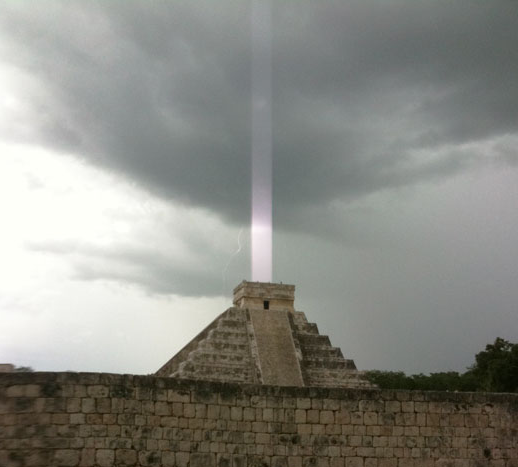
\includegraphics[width=200px]{imagenes/piramide.png}
	\caption{Pirámide}
\end{figure}
\begin{figure}
	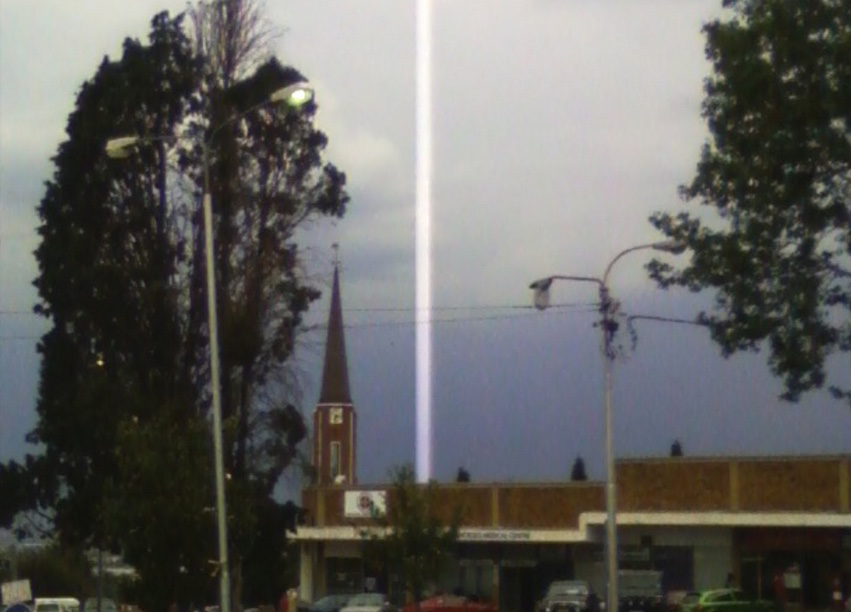
\includegraphics[width=200px]{imagenes/iglesia.png}
	\caption{Iglesia}
\end{figure}

    \hypertarget{soluciuxf3n-propuesta}{%
\section{Solución propuesta}\label{soluciuxf3n-propuesta}}

La solución propuesta se basa en acotar el artefacto y aplicarle una
compensación de exposición dadas las características propias definidas
en el apartado anterior.

Se ha seguido una aproximación de tipo espacial, se trata de delimitar
correctamente los píxeles donde se produce el artefacto para que la
corrección no afecta a otras zonas de la imagen.

\hypertarget{acotaciuxf3n-de-la-franja}{%
\subsection{Acotación de la franja}\label{acotaciuxf3n-de-la-franja}}

La zona del rayo sobreexpuesta (que denominaremos \emph{franja}) es
siempre vertical y tiene una columna de inicio y otra de final. Para
ello, en un primer momento, se intentó delimitar las columnas utilizando
un sumatorio de todos los \textbf{máximos} que aparecen en la fotografía
y aplicando una detección de máximos (picos) similar al ejemplo mostrado
en las lecciones magistrales de la asignatura. Para algunos casos
particulares esta solución funcionaba correctamente pero en imágenes
donde aparecian otros máximos de luz o en los cuales el artefacto no
tenia tanto brillo no servían.

La solución adoptada es similar, pero nos basamos en detectar los
\textbf{gradientes de exposición} que ocurren en la imagen. Además, para
eliminar posibles \textbf{falsos gradientes} que no corresponden al
artefacto, y aprovechando que la franja es vertical, aplicamos a cada
línea de la imagen el cálculo de sus gradientes y realizando un
sumatorio de todas las líneas para calcular cuales son las columnas que
poseen un mayor número en el gradiente. Para una gran cantidad de casos,
este método delimita correctamente las columnas de píxeles entre las que
se produce la franja del artefacto.

Por otro lado, también se debe de acotar la franja de manera vertical,
ya que el artefacto suele ocurrir en la parte del cielo (superior de la
franja), y no en el primer plano de la imagen (inferior de la franja).
Se ha vuelto a utilizar el método anterior para calcular el cambio mayor
de gradiente, pero en este caso, se ha realizado según sus columnas. Se
ha calculado el gradiente por cada columna, y se ha realizado un
sumatorio de todas ellas para ver dónde se produce el gradiente
acumulado mayor. Este será establecido como el final del artefacto.

\hypertarget{disminuciuxf3n-de-la-exposiciuxf3n}{%
\subsection{Disminución de la
exposición}\label{disminuciuxf3n-de-la-exposiciuxf3n}}

En un primer momento se intento aplicar una corrección constante a toda
la franja para disminuir la exposición a la luz producida. En cambio,
tal y como hemos definido en las características del artefacto, este no
es constante ni de manera horizontal ni de manera vertical.

Se ha aplicado una metodología para realizar una corrección que suavice
el efecto del cambio que se produce en la vertical de la franja. Para
ello, por cada fila de píxeles que hay en la franja, se calcula su
media, y se corrigen en grupo con la diferencia de la media del mismo
número de píxeles que el ancho de la franja tomados a un lado de la
misma.

Se elige el lado \textbf{izquierdo o derecho} de la franja para calcular
la média de valores de intensidad de un número de píxeles igual a la
anchura de la franja, en base a la diferencia de su media con la media
de los píxeles de la franja, y tomando aquellos que tienen una
diferencia menor. Con esta elección se intenta evitar algunas zonas que
son cercanas a la franja pero que no corresponden a una parte de cielo
similar a donde se produce el evento, por ejemplo, alteradas por un
árbol alto o una farola. Además, para mejorar el cálculo de la media y
la corrección, se eliminarán outliers que puedan ocurrir en esa franja.
Para la eliminación de los outliers, se ha cogido el vector
correspondiente de la franja de cada fila, y se han buscado valores que
se desvíen en dos desviaciones típicas de la media.

La corrección de la exposición se aplican por cada canal de color por
separado. Esto produce además que haya una corrección de lo que sería
las diferentes posibles cambios en la temperatura de la luz iluminando
el cielo.

    \hypertarget{ejecuciuxf3n-comentada-del-algoritmo}{%
\section{Ejecución comentada del
algoritmo}\label{ejecuciuxf3n-comentada-del-algoritmo}}

\hypertarget{libreruxedas-necesarias}{%
\subsection{Librerías necesarias}\label{libreruxedas-necesarias}}

Cargamos todas las librerías que necesitaremos para resolver la
actividad.

\begin{itemize}
\tightlist
\item
  numpy: Trabajo con arrays
\item
  matplotlib: Representación de funciones e imágenes
\item
  opencv: Carga de imágenes y obtención de propiedades y canales de la
  misma
\item
  scipy: Librería para operaciones matemáticas
\item
  operator: Librería para trabajar con sus operadores
\end{itemize}

    \begin{tcolorbox}[breakable, size=fbox, boxrule=1pt, pad at break*=1mm,colback=cellbackground, colframe=cellborder]
\prompt{In}{incolor}{1}{\boxspacing}
\begin{Verbatim}[commandchars=\\\{\}]
\PY{c+c1}{\PYZsh{} Importamos librerias necesarias }
\PY{k+kn}{import} \PY{n+nn}{numpy} \PY{k}{as} \PY{n+nn}{np}
\PY{k+kn}{import} \PY{n+nn}{matplotlib}\PY{n+nn}{.}\PY{n+nn}{pyplot} \PY{k}{as} \PY{n+nn}{plt}
\PY{k+kn}{import} \PY{n+nn}{cv2}
\PY{k+kn}{from} \PY{n+nn}{scipy}\PY{n+nn}{.}\PY{n+nn}{signal} \PY{k+kn}{import} \PY{n}{argrelextrema}
\PY{k+kn}{import} \PY{n+nn}{operator}
\end{Verbatim}
\end{tcolorbox}

    \hypertarget{definiciuxf3n-de-funciones}{%
\subsection{Definición de funciones}\label{definiciuxf3n-de-funciones}}

Definición de funciones necesarias para realizar las diferentes acciones
de resolución.

    \begin{tcolorbox}[breakable, size=fbox, boxrule=1pt, pad at break*=1mm,colback=cellbackground, colframe=cellborder]
\prompt{In}{incolor}{30}{\boxspacing}
\begin{Verbatim}[commandchars=\\\{\}]
\PY{k}{def} \PY{n+nf}{imshow}\PY{p}{(}\PY{n}{img}\PY{p}{,} \PY{n}{title}\PY{o}{=}\PY{k+kc}{None}\PY{p}{)}\PY{p}{:}
    \PY{l+s+sd}{\PYZdq{}\PYZdq{}\PYZdq{}}
\PY{l+s+sd}{    Función para representar una imagen}
\PY{l+s+sd}{    }
\PY{l+s+sd}{    Args:}
\PY{l+s+sd}{        img (Numpy Array): Imagen en formato numpy array}
\PY{l+s+sd}{        title (String): Texto del título del plot}
\PY{l+s+sd}{    \PYZdq{}\PYZdq{}\PYZdq{}}
    \PY{n}{fig} \PY{p}{,} \PY{n}{ax} \PY{o}{=} \PY{n}{plt}\PY{o}{.}\PY{n}{subplots}\PY{p}{(}\PY{n}{figsize} \PY{o}{=} \PY{p}{(}\PY{l+m+mi}{7}\PY{p}{,}\PY{l+m+mi}{7}\PY{p}{)}\PY{p}{)}
    \PY{n}{ax}\PY{o}{.}\PY{n}{imshow}\PY{p}{(}\PY{n}{img}\PY{p}{,} \PY{n}{cmap}\PY{o}{=}\PY{n}{plt}\PY{o}{.}\PY{n}{cm}\PY{o}{.}\PY{n}{gray}\PY{p}{)}
    \PY{n}{ax}\PY{o}{.}\PY{n}{set\PYZus{}xticks}\PY{p}{(}\PY{p}{[}\PY{p}{]}\PY{p}{)}
    \PY{n}{ax}\PY{o}{.}\PY{n}{set\PYZus{}yticks}\PY{p}{(}\PY{p}{[}\PY{p}{]}\PY{p}{)}
    \PY{k}{if} \PY{p}{(}\PY{n}{title} \PY{o+ow}{is} \PY{o+ow}{not} \PY{k+kc}{None}\PY{p}{)}\PY{p}{:}
        \PY{n}{plt}\PY{o}{.}\PY{n}{title}\PY{p}{(}\PY{n}{title}\PY{p}{)}
    \PY{n}{plt}\PY{o}{.}\PY{n}{show}\PY{p}{(}\PY{p}{)}
    
    
\PY{k}{def} \PY{n+nf}{maxOfRow}\PY{p}{(}\PY{n}{row}\PY{p}{)}\PY{p}{:}
    \PY{l+s+sd}{\PYZdq{}\PYZdq{}\PYZdq{}}
\PY{l+s+sd}{    Función para devolver los máximos de un vector de valores}
\PY{l+s+sd}{    }
\PY{l+s+sd}{    Args:}
\PY{l+s+sd}{        row (Numpy Array): Vector de valores sobre el que calcular}
\PY{l+s+sd}{                           el máximo.}
\PY{l+s+sd}{        }
\PY{l+s+sd}{    Return: Numpy array con los valores máximos}
\PY{l+s+sd}{    \PYZdq{}\PYZdq{}\PYZdq{}}
    \PY{n}{m} \PY{o}{=} \PY{n+nb}{max}\PY{p}{(}\PY{n}{row}\PY{p}{)}
    \PY{k}{return} \PY{n}{np}\PY{o}{.}\PY{n}{array}\PY{p}{(}\PY{p}{[}\PY{n}{i} \PY{k}{for} \PY{n}{i}\PY{p}{,} \PY{n}{j} \PY{o+ow}{in} \PY{n+nb}{enumerate}\PY{p}{(}\PY{n}{row}\PY{p}{)} \PY{k}{if} \PY{n}{j} \PY{o}{==} \PY{n}{m}\PY{p}{]}\PY{p}{)}


\PY{k}{def} \PY{n+nf}{fixImage}\PY{p}{(}\PY{n}{img}\PY{p}{,} \PY{n}{\PYZus{}from}\PY{p}{,} \PY{n}{\PYZus{}to}\PY{p}{,} \PY{n}{band}\PY{p}{)}\PY{p}{:}
    \PY{l+s+sd}{\PYZdq{}\PYZdq{}\PYZdq{}}
\PY{l+s+sd}{    Función para corregir la franja en la que se produce el artefacto en una imagen}
\PY{l+s+sd}{    }
\PY{l+s+sd}{    Args:}
\PY{l+s+sd}{        img (Numpy Array): Imagen sobre la que corregir artefacto}
\PY{l+s+sd}{        \PYZus{}from (Int): Valor del píxel de origen de la franja}
\PY{l+s+sd}{        \PYZus{}to (Int): Valor del píxel de finalización de la franja}
\PY{l+s+sd}{        band (Int): Banda sobre la que se realiza la corrección}
\PY{l+s+sd}{        }
\PY{l+s+sd}{    Return: Tupla (Numpy Array con la imagen modificada y corregida,}
\PY{l+s+sd}{                   gradientes de la banda)}
\PY{l+s+sd}{    \PYZdq{}\PYZdq{}\PYZdq{}}
    \PY{c+c1}{\PYZsh{}\PYZsh{}\PYZsh{}editar la franja}
    \PY{n}{modifiedImg} \PY{o}{=} \PY{n}{np}\PY{o}{.}\PY{n}{array}\PY{p}{(}\PY{n}{img}\PY{p}{)}
    
    \PY{n}{gradients} \PY{o}{=} \PY{n}{np}\PY{o}{.}\PY{n}{zeros}\PY{p}{(}\PY{n+nb}{len}\PY{p}{(}\PY{n}{img}\PY{p}{[}\PY{p}{:}\PY{p}{,}\PY{l+m+mi}{0}\PY{p}{]}\PY{p}{)}\PY{p}{)}

    \PY{k}{for} \PY{n}{j} \PY{o+ow}{in} \PY{n+nb}{range}\PY{p}{(}\PY{n}{\PYZus{}from}\PY{p}{,} \PY{n}{\PYZus{}to}\PY{p}{)}\PY{p}{:}
        \PY{n}{gradients} \PY{o}{=} \PY{p}{[}\PY{n}{x} \PY{o}{+} \PY{n}{y} \PY{k}{for} \PY{n}{x}\PY{p}{,} \PY{n}{y} \PY{o+ow}{in} \PY{n+nb}{zip}\PY{p}{(}\PY{n}{gradients}\PY{p}{,} \PY{n}{np}\PY{o}{.}\PY{n}{gradient}\PY{p}{(}\PY{n}{img}\PY{p}{[}\PY{p}{:}\PY{p}{,}\PY{n}{j}\PY{p}{]}\PY{p}{)}\PY{p}{)}\PY{p}{]}           
    
    \PY{n}{rowLimit} \PY{o}{=} \PY{n+nb}{min}\PY{p}{(}\PY{n}{gradients}\PY{p}{)}
    \PY{n}{rowLimit} \PY{o}{=} \PY{p}{[}\PY{n}{i} \PY{k}{for} \PY{n}{i}\PY{p}{,} \PY{n}{j} \PY{o+ow}{in} \PY{n+nb}{enumerate}\PY{p}{(}\PY{n}{gradients}\PY{p}{)} \PY{k}{if} \PY{n}{j} \PY{o}{==} \PY{n}{rowLimit}\PY{p}{]}\PY{p}{[}\PY{l+m+mi}{0}\PY{p}{]}
    \PY{k}{for} \PY{n}{i} \PY{o+ow}{in} \PY{n+nb}{range}\PY{p}{(}\PY{n}{rowLimit}\PY{p}{)}\PY{p}{:}
        \PY{n}{row} \PY{o}{=} \PY{n}{img}\PY{p}{[}\PY{n}{i}\PY{p}{,}\PY{p}{:}\PY{p}{]}
        \PY{n}{newRow} \PY{o}{=} \PY{n}{fixRow}\PY{p}{(}\PY{n}{row}\PY{p}{,} \PY{n}{\PYZus{}from}\PY{p}{,} \PY{n}{\PYZus{}to}\PY{p}{)}
        \PY{n}{modifiedImg}\PY{p}{[}\PY{n}{i}\PY{p}{,} \PY{n}{\PYZus{}from}\PY{p}{:}\PY{n}{\PYZus{}to}\PY{p}{]} \PY{o}{=} \PY{n}{newRow}
    
    \PY{k}{return} \PY{n}{modifiedImg}\PY{p}{,} \PY{n}{gradients}


\PY{k}{def} \PY{n+nf}{fixRow}\PY{p}{(}\PY{n}{row}\PY{p}{,} \PY{n}{\PYZus{}from}\PY{p}{,} \PY{n}{\PYZus{}to}\PY{p}{)}\PY{p}{:}
    \PY{l+s+sd}{\PYZdq{}\PYZdq{}\PYZdq{}}
\PY{l+s+sd}{    Función para corregir los valores de una fila de la imagen}
\PY{l+s+sd}{    }
\PY{l+s+sd}{    Args:}
\PY{l+s+sd}{        row (Numpy Array): Vector con los valores de la fila de la}
\PY{l+s+sd}{                           imagen a corregir}
\PY{l+s+sd}{        \PYZus{}from (Int): Posición del píxel de inicio desde el que corregir}
\PY{l+s+sd}{        \PYZus{}to (Int): Posición del píxel de final hasta el que corregir }
\PY{l+s+sd}{    }
\PY{l+s+sd}{    Return: Numpy Array de valores modificados con la fila cambiada}
\PY{l+s+sd}{    \PYZdq{}\PYZdq{}\PYZdq{}}
    \PY{c+c1}{\PYZsh{} Elegimos el lado que sirve de base para hacer la correccion}
    \PY{c+c1}{\PYZsh{} Eliminan outliers para sacar la media de cada tramo}
    \PY{n}{rangeLen} \PY{o}{=} \PY{n}{\PYZus{}to} \PY{o}{\PYZhy{}} \PY{n}{\PYZus{}from}
    
    \PY{n}{leftSliceCorrect} \PY{o}{=} \PY{n}{row}\PY{p}{[}\PY{n}{\PYZus{}from}\PY{o}{\PYZhy{}}\PY{n}{rangeLen}\PY{p}{:}\PY{n}{\PYZus{}to}\PY{o}{\PYZhy{}}\PY{n}{rangeLen}\PY{p}{]}
    \PY{n}{leftSliceCorrectValue} \PY{o}{=} \PY{n}{np}\PY{o}{.}\PY{n}{mean}\PY{p}{(}\PY{n}{deleteOutlier}\PY{p}{(}\PY{n}{leftSliceCorrect}\PY{p}{)}\PY{p}{)}
    \PY{n}{rightSliceCorrect} \PY{o}{=} \PY{n}{row}\PY{p}{[}\PY{n}{\PYZus{}from}\PY{o}{+}\PY{n}{rangeLen}\PY{p}{:}\PY{n}{\PYZus{}to}\PY{o}{+}\PY{n}{rangeLen}\PY{p}{]}
    \PY{n}{rightSliceCorrectValue} \PY{o}{=} \PY{n}{np}\PY{o}{.}\PY{n}{mean}\PY{p}{(}\PY{n}{deleteOutlier}\PY{p}{(}\PY{n}{rightSliceCorrect}\PY{p}{)}\PY{p}{)}

    \PY{n}{artefactSlice} \PY{o}{=} \PY{n}{row}\PY{p}{[}\PY{n}{\PYZus{}from}\PY{p}{:}\PY{n}{\PYZus{}to}\PY{p}{]}
    \PY{n}{artefactSliceValue} \PY{o}{=}\PY{n}{np}\PY{o}{.}\PY{n}{mean}\PY{p}{(}\PY{n}{deleteOutlier}\PY{p}{(}\PY{n}{artefactSlice}\PY{p}{)}\PY{p}{)}
    
    \PY{n}{dLeft} \PY{o}{=} \PY{n+nb}{abs}\PY{p}{(}\PY{n}{leftSliceCorrectValue} \PY{o}{\PYZhy{}} \PY{n}{artefactSliceValue}\PY{p}{)}
    \PY{n}{dRight} \PY{o}{=} \PY{n+nb}{abs}\PY{p}{(}\PY{n}{rightSliceCorrectValue} \PY{o}{\PYZhy{}} \PY{n}{artefactSliceValue}\PY{p}{)}
    
    \PY{k}{if} \PY{p}{(}\PY{n}{dRight}\PY{o}{\PYZlt{}}\PY{n}{dLeft}\PY{p}{)}\PY{p}{:}
        \PY{c+c1}{\PYZsh{}lado = \PYZdq{}derecho\PYZdq{}}
        \PY{n}{valueSlideCorrection} \PY{o}{=} \PY{n}{rightSliceCorrectValue}
    \PY{k}{else}\PY{p}{:}
        \PY{c+c1}{\PYZsh{}lado = \PYZdq{}izquierdo\PYZdq{}}
        \PY{n}{valueSlideCorrection} \PY{o}{=} \PY{n}{leftSliceCorrectValue}
            
    \PY{n}{diff} \PY{o}{=} \PY{n}{artefactSliceValue} \PY{o}{\PYZhy{}} \PY{n}{valueSlideCorrection}

    \PY{c+c1}{\PYZsh{}print (\PYZdq{}Diferencia:\PYZdq{}, diff,}
    \PY{c+c1}{\PYZsh{}       \PYZdq{}lado: \PYZdq{}, lado,}
    \PY{c+c1}{\PYZsh{}       \PYZdq{}izq: \PYZdq{}, leftSliceCorrectValue,}
    \PY{c+c1}{\PYZsh{}       \PYZdq{}mid: \PYZdq{}, artefactSliceValue,}
    \PY{c+c1}{\PYZsh{}       \PYZdq{}der: \PYZdq{}, rightSliceCorrectValue,}
    \PY{c+c1}{\PYZsh{}       \PYZdq{}Diferencia: \PYZdq{}, diff)}
    
    \PY{n}{newRow} \PY{o}{=} \PY{n}{row}\PY{p}{[}\PY{n}{\PYZus{}from}\PY{p}{:}\PY{n}{\PYZus{}to}\PY{p}{]} \PY{o}{\PYZhy{}} \PY{n}{diff}
    
    \PY{c+c1}{\PYZsh{}Correccion de maximos minimos en la imagen}
    \PY{n}{newRow}\PY{p}{[}\PY{n}{newRow} \PY{o}{\PYZlt{}} \PY{l+m+mi}{0}\PY{p}{]} \PY{o}{=} \PY{l+m+mi}{0}
    \PY{n}{newRow}\PY{p}{[}\PY{n}{newRow} \PY{o}{\PYZgt{}} \PY{l+m+mi}{255}\PY{p}{]} \PY{o}{=} \PY{l+m+mi}{255}  
    
    \PY{k}{return} \PY{n}{newRow}
    
    
\PY{k}{def} \PY{n+nf}{deleteOutlier}\PY{p}{(}\PY{n}{an\PYZus{}array}\PY{p}{)}\PY{p}{:}
    \PY{l+s+sd}{\PYZdq{}\PYZdq{}\PYZdq{}}
\PY{l+s+sd}{    Función para eliminar los posibles outliers de nuestro vector de valores}
\PY{l+s+sd}{    }
\PY{l+s+sd}{    Args:}
\PY{l+s+sd}{        an\PYZus{}array (Numpy Array): Valores sobre los que corregir los outliers}
\PY{l+s+sd}{        }
\PY{l+s+sd}{    Return: Numpy Array Vector sin los outliers}
\PY{l+s+sd}{    \PYZdq{}\PYZdq{}\PYZdq{}}
    \PY{n}{mean} \PY{o}{=} \PY{n}{np}\PY{o}{.}\PY{n}{mean}\PY{p}{(}\PY{n}{an\PYZus{}array}\PY{p}{)}
    \PY{n}{standard\PYZus{}deviation} \PY{o}{=} \PY{n}{np}\PY{o}{.}\PY{n}{std}\PY{p}{(}\PY{n}{an\PYZus{}array}\PY{p}{)}
    \PY{n}{distance\PYZus{}from\PYZus{}mean} \PY{o}{=} \PY{n+nb}{abs}\PY{p}{(}\PY{n}{an\PYZus{}array} \PY{o}{\PYZhy{}} \PY{n}{mean}\PY{p}{)}
    \PY{n}{max\PYZus{}deviations} \PY{o}{=} \PY{l+m+mi}{2}
    \PY{n}{not\PYZus{}outlier} \PY{o}{=} \PY{n}{distance\PYZus{}from\PYZus{}mean} \PY{o}{\PYZlt{}} \PY{n}{max\PYZus{}deviations} \PY{o}{*} \PY{n}{standard\PYZus{}deviation}
    \PY{n}{no\PYZus{}outliers} \PY{o}{=} \PY{n}{an\PYZus{}array}\PY{p}{[}\PY{n}{not\PYZus{}outlier}\PY{p}{]}
    \PY{k}{return} \PY{n}{no\PYZus{}outliers} 


\PY{k}{def} \PY{n+nf}{detectBand}\PY{p}{(}\PY{n}{gradients}\PY{p}{)}\PY{p}{:}
    \PY{l+s+sd}{\PYZdq{}\PYZdq{}\PYZdq{}}
\PY{l+s+sd}{    Función para detectar la franja de valores atípicos}
\PY{l+s+sd}{    }
\PY{l+s+sd}{    Args:}
\PY{l+s+sd}{        gradients (List): Listado de valores gradientes}
\PY{l+s+sd}{        }
\PY{l+s+sd}{    Return: Tuple con los valores máximo y mínimo de gradiente}
\PY{l+s+sd}{    \PYZdq{}\PYZdq{}\PYZdq{}}
    \PY{c+c1}{\PYZsh{}detecta la franja en una línea dado un máximo}
    
    \PY{n}{max\PYZus{}g} \PY{o}{=} \PY{n+nb}{max}\PY{p}{(}\PY{n}{gradients}\PY{p}{)}
    \PY{n}{maximum\PYZus{}gradient} \PY{o}{=} \PY{p}{[}\PY{n}{i} \PY{k}{for} \PY{n}{i}\PY{p}{,} \PY{n}{j} \PY{o+ow}{in} \PY{n+nb}{enumerate}\PY{p}{(}\PY{n}{gradients}\PY{p}{)} \PY{k}{if} \PY{n}{j} \PY{o}{==} \PY{n}{max\PYZus{}g}\PY{p}{]}\PY{p}{[}\PY{l+m+mi}{0}\PY{p}{]}
    \PY{n}{min\PYZus{}g} \PY{o}{=} \PY{n+nb}{min}\PY{p}{(}\PY{n}{gradients}\PY{p}{)}
    \PY{n}{minimum\PYZus{}gradiente} \PY{o}{=} \PY{p}{[}\PY{n}{i} \PY{k}{for} \PY{n}{i}\PY{p}{,} \PY{n}{j} \PY{o+ow}{in} \PY{n+nb}{enumerate}\PY{p}{(}\PY{n}{gradients}\PY{p}{)} \PY{k}{if} \PY{n}{j} \PY{o}{==} \PY{n}{min\PYZus{}g}\PY{p}{]}\PY{p}{[}\PY{l+m+mi}{0}\PY{p}{]}
    \PY{k}{return} \PY{n}{maximum\PYZus{}gradient}\PY{p}{,} \PY{n}{minimum\PYZus{}gradiente}


\PY{k}{def} \PY{n+nf}{getGrandientSumBands}\PY{p}{(}\PY{n}{img}\PY{p}{)}\PY{p}{:}
    \PY{l+s+sd}{\PYZdq{}\PYZdq{}\PYZdq{}}
\PY{l+s+sd}{    Función para detectar las bandas mediante suma de gradientes}
\PY{l+s+sd}{    }
\PY{l+s+sd}{    Args:}
\PY{l+s+sd}{        img (Numpy Array): Imagen sobre la que detectar las franjas}
\PY{l+s+sd}{        }
\PY{l+s+sd}{    Return: Tupla (maximum\PYZus{}gradient, minimum\PYZus{}gradiente, gradients)}
\PY{l+s+sd}{    \PYZdq{}\PYZdq{}\PYZdq{}}
    \PY{n}{nRows} \PY{o}{=} \PY{n}{img}\PY{o}{.}\PY{n}{shape}\PY{p}{[}\PY{l+m+mi}{0}\PY{p}{]}
    \PY{n}{gradients} \PY{o}{=} \PY{n}{np}\PY{o}{.}\PY{n}{zeros}\PY{p}{(}\PY{n+nb}{len}\PY{p}{(}\PY{n}{img}\PY{p}{[}\PY{l+m+mi}{0}\PY{p}{,}\PY{p}{:}\PY{p}{,}\PY{l+m+mi}{0}\PY{p}{]}\PY{p}{)}\PY{p}{)}
    
    \PY{k}{for} \PY{n}{i} \PY{o+ow}{in} \PY{n+nb}{range}\PY{p}{(}\PY{l+m+mi}{3}\PY{p}{)}\PY{p}{:}  
        \PY{k}{for} \PY{n}{j} \PY{o+ow}{in} \PY{n+nb}{range}\PY{p}{(}\PY{n}{nRows}\PY{p}{)}\PY{p}{:}
            \PY{n}{gradients} \PY{o}{=} \PY{p}{[}\PY{n}{x} \PY{o}{+} \PY{n}{y} \PY{k}{for} \PY{n}{x}\PY{p}{,} \PY{n}{y} \PY{o+ow}{in} \PY{n+nb}{zip}\PY{p}{(}\PY{n}{gradients}\PY{p}{,} \PY{n}{np}\PY{o}{.}\PY{n}{gradient}\PY{p}{(}\PY{n}{img}\PY{p}{[}\PY{n}{j}\PY{p}{,}\PY{p}{:}\PY{p}{,}\PY{n}{i}\PY{p}{]}\PY{p}{)}\PY{p}{)}\PY{p}{]}            

    \PY{k}{return} \PY{n}{detectBand}\PY{p}{(}\PY{n}{np}\PY{o}{.}\PY{n}{array}\PY{p}{(}\PY{n}{gradients}\PY{p}{)}\PY{p}{)}\PY{p}{,} \PY{n}{gradients}
\end{Verbatim}
\end{tcolorbox}

    \hypertarget{cuxf3digo-de-ejecuciuxf3n}{%
\subsection{Código de ejecución}\label{cuxf3digo-de-ejecuciuxf3n}}

Código en el que se ejecutan las funciones sobre las imágenes con el
artefacto para detectar y corregir el mismo.

    \begin{tcolorbox}[breakable, size=fbox, boxrule=1pt, pad at break*=1mm,colback=cellbackground, colframe=cellborder]
\prompt{In}{incolor}{31}{\boxspacing}
\begin{Verbatim}[commandchars=\\\{\}]
\PY{k+kn}{from} \PY{n+nn}{IPython}\PY{n+nn}{.}\PY{n+nn}{core}\PY{n+nn}{.}\PY{n+nn}{display} \PY{k+kn}{import} \PY{n}{display}\PY{p}{,} \PY{n}{HTML}

\PY{c+c1}{\PYZsh{} Cargamos los paths de las imgs}
\PY{n}{imgs\PYZus{}path} \PY{o}{=} \PY{p}{[}\PY{l+s+s1}{\PYZsq{}}\PY{l+s+s1}{imagenes/piramide.png}\PY{l+s+s1}{\PYZsq{}}\PY{p}{,} 
             \PY{l+s+s1}{\PYZsq{}}\PY{l+s+s1}{imagenes/iglesia.png}\PY{l+s+s1}{\PYZsq{}}\PY{p}{]}
\PY{n}{display}\PY{p}{(}\PY{n}{HTML}\PY{p}{(}\PY{l+s+s1}{\PYZsq{}}\PY{l+s+s1}{\PYZlt{}h1\PYZgt{}Corrección de imagenes\PYZlt{}/h1\PYZgt{}}\PY{l+s+s1}{\PYZsq{}}\PY{p}{)}\PY{p}{)}
\PY{c+c1}{\PYZsh{} Recorremos las imgs para realizar la deteccion y correccion a cada una}
\PY{k}{for} \PY{n}{img\PYZus{}path} \PY{o+ow}{in} \PY{n}{imgs\PYZus{}path}\PY{p}{:}
    \PY{n}{display}\PY{p}{(}\PY{n}{HTML}\PY{p}{(}\PY{l+s+s1}{\PYZsq{}}\PY{l+s+s1}{\PYZlt{}h2\PYZgt{}Imagen: }\PY{l+s+s1}{\PYZsq{}}\PY{o}{+} \PY{n}{img\PYZus{}path} \PY{o}{+} \PY{l+s+s1}{\PYZsq{}}\PY{l+s+s1}{\PYZlt{}/h2\PYZgt{}}\PY{l+s+s1}{\PYZsq{}}\PY{p}{)}\PY{p}{)}
    \PY{c+c1}{\PYZsh{} cargamos la img}
    \PY{n}{originalImg} \PY{o}{=} \PY{n}{cv2}\PY{o}{.}\PY{n}{imread}\PY{p}{(}\PY{n}{img\PYZus{}path}\PY{p}{)}

    \PY{c+c1}{\PYZsh{} obtenemos las dimensiones de la img}
    \PY{n}{h}\PY{p}{,} \PY{n}{w}\PY{p}{,} \PY{n}{b} \PY{o}{=} \PY{n}{originalImg}\PY{o}{.}\PY{n}{shape}
    
    \PY{c+c1}{\PYZsh{} Cambiamos de BGR a RGB}
    \PY{n}{originalImg} \PY{o}{=} \PY{n}{cv2}\PY{o}{.}\PY{n}{cvtColor}\PY{p}{(}\PY{n}{originalImg}\PY{p}{,} \PY{n}{cv2}\PY{o}{.}\PY{n}{COLOR\PYZus{}BGR2RGB}\PY{p}{)}
    \PY{c+c1}{\PYZsh{} Creamos una copia de la imagen para modificar sobre ella el artefacto}
    \PY{n}{fixedImg} \PY{o}{=} \PY{n}{np}\PY{o}{.}\PY{n}{array}\PY{p}{(}\PY{n}{originalImg}\PY{p}{)}
    
    \PY{n}{f}\PY{p}{,} \PY{n}{plots} \PY{o}{=} \PY{n}{plt}\PY{o}{.}\PY{n}{subplots}\PY{p}{(}\PY{n}{nrows}\PY{o}{=}\PY{l+m+mi}{2}\PY{p}{,} \PY{n}{ncols}\PY{o}{=}\PY{l+m+mi}{2}\PY{p}{,} \PY{n}{figsize}\PY{o}{=}\PY{p}{(}\PY{l+m+mi}{15}\PY{p}{,}\PY{l+m+mi}{15}\PY{p}{)}\PY{p}{)}
    
    \PY{c+c1}{\PYZsh{} Obtenemos el origen y final del artefacto}
    \PY{n}{f\PYZus{}t}\PY{p}{,} \PY{n}{gradient} \PY{o}{=} \PY{n}{getGrandientSumBands}\PY{p}{(}\PY{n}{originalImg}\PY{p}{)}
    \PY{n}{\PYZus{}from} \PY{o}{=} \PY{n}{f\PYZus{}t}\PY{p}{[}\PY{l+m+mi}{0}\PY{p}{]}
    \PY{n}{\PYZus{}to} \PY{o}{=} \PY{n}{f\PYZus{}t}\PY{p}{[}\PY{l+m+mi}{1}\PY{p}{]}
    
    \PY{n}{plots}\PY{p}{[}\PY{l+m+mi}{0}\PY{p}{]}\PY{p}{[}\PY{l+m+mi}{0}\PY{p}{]}\PY{o}{.}\PY{n}{plot}\PY{p}{(}\PY{n}{gradient}\PY{p}{)}
    \PY{n}{plots}\PY{p}{[}\PY{l+m+mi}{0}\PY{p}{]}\PY{p}{[}\PY{l+m+mi}{0}\PY{p}{]}\PY{o}{.}\PY{n}{title}\PY{o}{.}\PY{n}{set\PYZus{}text}\PY{p}{(}\PY{l+s+s1}{\PYZsq{}}\PY{l+s+s1}{Sumatorio de gradientes}\PY{l+s+s1}{\PYZsq{}}\PY{p}{)}
    
    \PY{c+c1}{\PYZsh{} Recorremos las bandas para corregir en cada una de ellas el artefacto}
    \PY{k}{for} \PY{n}{i} \PY{o+ow}{in} \PY{n+nb}{range}\PY{p}{(}\PY{n}{b}\PY{p}{)}\PY{p}{:}    
        \PY{n}{fixedImg}\PY{p}{[}\PY{p}{:}\PY{p}{,}\PY{p}{:}\PY{p}{,}\PY{n}{i}\PY{p}{]}\PY{p}{,} \PY{n}{gradient} \PY{o}{=} \PY{n}{fixImage}\PY{p}{(}\PY{n}{originalImg}\PY{p}{[}\PY{p}{:}\PY{p}{,}\PY{p}{:}\PY{p}{,}\PY{n}{i}\PY{p}{]}\PY{p}{,} \PY{n}{\PYZus{}from}\PY{p}{,} \PY{n}{\PYZus{}to}\PY{p}{,} \PY{n}{i}\PY{p}{)}
        \PY{k}{if} \PY{n}{i} \PY{o}{==} \PY{l+m+mi}{0}\PY{p}{:}
            \PY{n}{plots}\PY{p}{[}\PY{l+m+mi}{0}\PY{p}{]}\PY{p}{[}\PY{l+m+mi}{1}\PY{p}{]}\PY{o}{.}\PY{n}{plot}\PY{p}{(}\PY{n}{gradient}\PY{p}{)}
            \PY{n}{plots}\PY{p}{[}\PY{l+m+mi}{0}\PY{p}{]}\PY{p}{[}\PY{l+m+mi}{1}\PY{p}{]}\PY{o}{.}\PY{n}{title}\PY{o}{.}\PY{n}{set\PYZus{}text}\PY{p}{(}\PY{l+s+s2}{\PYZdq{}}\PY{l+s+s2}{Gradientes en la banda: }\PY{l+s+s2}{\PYZdq{}}\PY{o}{+} \PY{n+nb}{str}\PY{p}{(}\PY{n}{i}\PY{p}{)}\PY{p}{)}
        \PY{k}{elif} \PY{n}{i}\PY{o}{==}\PY{l+m+mi}{1}\PY{p}{:}
            \PY{n}{plots}\PY{p}{[}\PY{l+m+mi}{1}\PY{p}{]}\PY{p}{[}\PY{l+m+mi}{0}\PY{p}{]}\PY{o}{.}\PY{n}{plot}\PY{p}{(}\PY{n}{gradient}\PY{p}{)}
            \PY{n}{plots}\PY{p}{[}\PY{l+m+mi}{1}\PY{p}{]}\PY{p}{[}\PY{l+m+mi}{0}\PY{p}{]}\PY{o}{.}\PY{n}{title}\PY{o}{.}\PY{n}{set\PYZus{}text}\PY{p}{(}\PY{l+s+s2}{\PYZdq{}}\PY{l+s+s2}{Gradientes en la banda: }\PY{l+s+s2}{\PYZdq{}}\PY{o}{+} \PY{n+nb}{str}\PY{p}{(}\PY{n}{i}\PY{p}{)}\PY{p}{)}
        \PY{k}{elif} \PY{n}{i}\PY{o}{==}\PY{l+m+mi}{2}\PY{p}{:}
            \PY{n}{plots}\PY{p}{[}\PY{l+m+mi}{1}\PY{p}{]}\PY{p}{[}\PY{l+m+mi}{1}\PY{p}{]}\PY{o}{.}\PY{n}{plot}\PY{p}{(}\PY{n}{gradient}\PY{p}{)}
            \PY{n}{plots}\PY{p}{[}\PY{l+m+mi}{1}\PY{p}{]}\PY{p}{[}\PY{l+m+mi}{1}\PY{p}{]}\PY{o}{.}\PY{n}{title}\PY{o}{.}\PY{n}{set\PYZus{}text}\PY{p}{(}\PY{l+s+s2}{\PYZdq{}}\PY{l+s+s2}{Gradientes en la banda: }\PY{l+s+s2}{\PYZdq{}}\PY{o}{+} \PY{n+nb}{str}\PY{p}{(}\PY{n}{i}\PY{p}{)}\PY{p}{)}
        
    \PY{n}{plt}\PY{o}{.}\PY{n}{show}\PY{p}{(}\PY{p}{)}
    
    \PY{c+c1}{\PYZsh{} Mostramos la imagen original y la arreglada}
    \PY{n}{f}\PY{p}{,} \PY{n}{plots} \PY{o}{=} \PY{n}{plt}\PY{o}{.}\PY{n}{subplots}\PY{p}{(}\PY{n}{ncols}\PY{o}{=}\PY{l+m+mi}{2}\PY{p}{,} \PY{n}{figsize}\PY{o}{=}\PY{p}{(}\PY{l+m+mi}{15}\PY{p}{,}\PY{l+m+mi}{15}\PY{p}{)}\PY{p}{)}
    
    \PY{n}{plots}\PY{p}{[}\PY{l+m+mi}{0}\PY{p}{]}\PY{o}{.}\PY{n}{imshow}\PY{p}{(}\PY{n}{originalImg}\PY{p}{)}
    \PY{n}{plots}\PY{p}{[}\PY{l+m+mi}{0}\PY{p}{]}\PY{o}{.}\PY{n}{set\PYZus{}xticks}\PY{p}{(}\PY{p}{[}\PY{p}{]}\PY{p}{)}\PY{p}{,} \PY{n}{plots}\PY{p}{[}\PY{l+m+mi}{0}\PY{p}{]}\PY{o}{.}\PY{n}{set\PYZus{}yticks}\PY{p}{(}\PY{p}{[}\PY{p}{]}\PY{p}{)}
    \PY{n}{plots}\PY{p}{[}\PY{l+m+mi}{0}\PY{p}{]}\PY{o}{.}\PY{n}{title}\PY{o}{.}\PY{n}{set\PYZus{}text}\PY{p}{(}\PY{l+s+s1}{\PYZsq{}}\PY{l+s+s1}{Imagen original: }\PY{l+s+s1}{\PYZsq{}}\PY{o}{+} \PY{n}{img\PYZus{}path}\PY{p}{)}
    \PY{n}{plots}\PY{p}{[}\PY{l+m+mi}{1}\PY{p}{]}\PY{o}{.}\PY{n}{imshow}\PY{p}{(}\PY{n}{fixedImg}\PY{p}{)}
    \PY{n}{plots}\PY{p}{[}\PY{l+m+mi}{1}\PY{p}{]}\PY{o}{.}\PY{n}{set\PYZus{}xticks}\PY{p}{(}\PY{p}{[}\PY{p}{]}\PY{p}{)}\PY{p}{,} \PY{n}{plots}\PY{p}{[}\PY{l+m+mi}{1}\PY{p}{]}\PY{o}{.}\PY{n}{set\PYZus{}yticks}\PY{p}{(}\PY{p}{[}\PY{p}{]}\PY{p}{)}
    \PY{n}{plots}\PY{p}{[}\PY{l+m+mi}{1}\PY{p}{]}\PY{o}{.}\PY{n}{title}\PY{o}{.}\PY{n}{set\PYZus{}text}\PY{p}{(}\PY{l+s+s1}{\PYZsq{}}\PY{l+s+s1}{Imagen corregida: }\PY{l+s+s1}{\PYZsq{}}\PY{o}{+} \PY{n}{img\PYZus{}path}\PY{p}{)}
    \PY{n}{plt}\PY{o}{.}\PY{n}{show}\PY{p}{(}\PY{p}{)}
\end{Verbatim}
\end{tcolorbox}


    
    \begin{center}
    \adjustimage{max size={0.9\linewidth}{0.9\paperheight}}{output_7_2.png}
    \end{center}
    { \hspace*{\fill} \\}
    
    \begin{center}
    \adjustimage{max size={0.9\linewidth}{0.9\paperheight}}{output_7_3.png}
    \end{center}
    { \hspace*{\fill} \\}
    

    
    \begin{center}
    \adjustimage{max size={0.9\linewidth}{0.9\paperheight}}{output_7_5.png}
    \end{center}
    { \hspace*{\fill} \\}
    
    \begin{center}
    \adjustimage{max size={0.9\linewidth}{0.9\paperheight}}{output_7_6.png}
    \end{center}
    { \hspace*{\fill} \\}
    
    \hypertarget{anuxe1lisis-de-resultados}{%
\section{Análisis de resultados}\label{anuxe1lisis-de-resultados}}

Los resultados en la imagen de la \textbf{pirámide} son muy
satisfactorios. Se puede comprobar que la corrección por filas produce
un buen resultado ya que las correcciones en la parte superior son
menores en tamaño que las de la parte inferior. La acotación de la
franja es correcta con la única excepción de las lineas en el borde de
las franja que tendrían que tratarse de forma independiente ya que se
comportan diferentes a las del centro de ella, de ahí que la corrección
produzca un efecto de oscurecimiento.

\begin{figure}
\centering
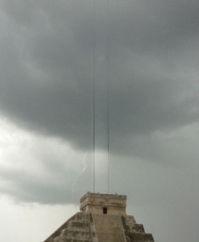
\includegraphics{imagenes/analisis_piramide1.png}
\caption{Análisis piramide}
\end{figure}

En la imagen de la \textbf{iglesia} los resultados son similares, con la
diferencia de que al ser la franja más pequeña, esos píxeles en sus
bordes cobran mayor importancia y producen que la corrección no sea del
todo acertada.

\hypertarget{conclusiones}{%
\section{Conclusiones}\label{conclusiones}}

Este artefacto es un artefacto muy cambiante ya que no es constante ni
su forma, ni su localización, ni su corrección. Incluso dentro del
propio artefacto se producen valores cambiantes que requieren de
implementar otras soluciones distintas para su corrección.

En esta implementación, se quedan fuera de la corrección algunas
características como reflejos producidos por la iluminación extra, que
estén en una zona que no es principalmente el cielo. En algunos casos
hay elementos como otras nubes que tapan parcialmente la franja de luz,
por lo que hace que haya artefactos que tienen una forma discontinua y
esto produce que la corrección del artefacto se corte antes de lo
previsto.

Además ocurren otros problemas en la localización de la franja, el
cambio de gradientes se puede producir en otros casos como son farolas o
postes de cemento, que al ser también verticales confunden al algoritmo
porque se comportan de forma similar al artefacto: franjas verticales
con una exposición mayor comparada con el cielo. En fotos nocturas con
gran cantidad de luces, también se puede producen cambios fuertes de
gradiente que dificultan la tarea.

Parece ser que para tener un algoritmo que cumpla correctamente para
corregir este artefacto y se cumpla bajo todas las condiciones posibles,
se deberían de juntar diferentes métodos para la detección de franjas
sobreexpuestas y correcciones no uniformes sobre ellas, tanto en
vertical como en horizontal, teniendo que tratar los píxeles de las
lines dentro de la franja como independientes. También mejorar el
cálculo del valor base para ajustar la exposición de la franja con la
del resto de la imagen para que siga manteniendo la forma.

    \hypertarget{referencias}{%
\section{Referencias}\label{referencias}}

https://www.metabunk.org/threads/why-people-are-suddenly-seeing-strange-beams-of-light-around-the-world-the-reddit-effect.6722/

https://en.wikipedia.org/wiki/Charge-coupled\_device

https://photo.stackexchange.com/questions/52969/why-is-there-a-vertical-bar-of-brighter-exposure-when-photographing-lightning

https://www.kite.com/python/answers/how-to-remove-outliers-from-a-numpy-array-in-python


    % Add a bibliography block to the postdoc
    
    
    
\end{document}
